\section{Inputs}

\begin{figure}[H]
\centering
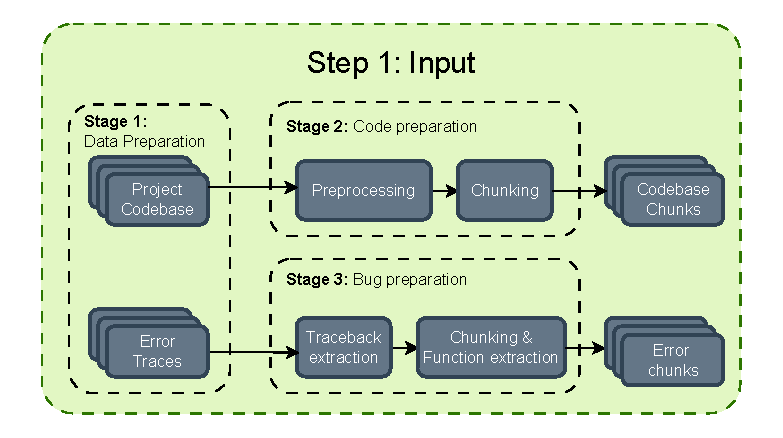
\includegraphics[width=1\columnwidth]{Figures/Step1_input.drawio.pdf}
\caption{Input processing}
\label{fig:step1_input}
\end{figure}


\subsection{Data Preparation}
Selecting an appropriate dataset is key to evaluating the pipeline. We use an enhanced version of the BugsInPy dataset \citep{aguilar2023reproducing}, which improves reproducibility by providing validated Docker environments for each bug. Projects were selected based on criteria that ensures diversity and sufficient number of bug cases. An overview of the selected projects is provided in Table~\ref{tab:bugsinpy_projects}

\begin{table}[H]
\centering
\begin{tabularx}{\textwidth}{lcccccccc}
\toprule
\textbf{Projects} & \textbf{Bugs} & \textbf{Avg. Trace LoC} & \textbf{Min. Trace LoC} & \textbf{Max. Trace LoC} & \textbf{File count} & \textbf{Avg. LoC} & \textbf{Min. LoC} & \textbf{Max. LoC} \\
\midrule
matplotlib & 23 & 91.2 & 49 & 232 & 762 & 244.3 & 1 & 8054 \\
pandas & 124 & 261.2 & 30 & 4375 & 297 & 602.8 & 1 & 11407 \\
youtube-dl & 31 & 26.3 & 2 & 56 & 809 & 159.7 & 4 & 3888 \\
luigi & 30 & 84.2 & 27 & 319 & 119 & 261.3 & 17 & 1647 \\
black & 19 & 138.5 & 18 & 591 & 23 & 4134.5 & 2 & 41441 \\
scrapy & 37 & 33.7 & 18 & 133 & 177 & 100.5 & 1 & 531 \\
thefuck & 30 & 84.8 & 27 & 363 & 198 & 33.6 & 1 & 338 \\
keras & 34 & 375.9 & 79 & 3476 & 135 & 362.8 & 1 & 4494 \\
ansible & 135 & 74.8 & 12 & 246 & 582 & 236.9 & 1 & 3446 \\
\bottomrule
\end{tabularx}
\caption{Projects chosen from BugsInPy dataset}
\label{tab:bugsinpy_projects}
\end{table}


\subsection{Code preparation}
Before embedding, we preprocess each project by cloning its repository and filtering out non-source files (e.g., tests, configuration scripts, and data). To handle long source files and improve semantic focus, we apply an AST-based chunking strategy. Using Python's built-in Abstract Syntax Tree (AST) module, we split each file into logical units corresponding to top-level classes and functions. This reduces noise from unrelated code and ensures that the resulting chunks are semantically meaningful.
\subsection{Bug preparation}
As part of bug preprocessing, we extract the relevant segments of each tracebacks by removing non-informative frames, such as logging calls and third-party utility layers. This refinement improves the overall success rate by 3\%. To ensure clear evaluation targets, we include only bugs where exactly one file is modified, based on the available ground truth.